\documentclass[11pt, oneside]{article}   	% use "amsart" instead of "article" for AMSLaTeX format
\usepackage{geometry}                		% See geometry.pdf to learn the layout options. There are lots.
\geometry{letterpaper}                   		% ... or a4paper or a5paper or ... 
%\geometry{landscape}                		% Activate for rotated page geometry
%\usepackage[parfill]{parskip}    		% Activate to begin paragraphs with an empty line rather than an indent
\usepackage{graphicx}				% Use pdf, png, jpg, or eps§ with pdflatex; use eps in DVI mode
								% TeX will automatically convert eps --> pdf in pdflatex		
\usepackage{amssymb}
\usepackage[latin1]{inputenc}
\usepackage{tikz}
\usepackage{graphicx}
\usetikzlibrary{shapes,arrows}

%SetFonts

%SetFonts


\title{Digit Recognizer}
\author{Terris Becker, Travis Barton}
%\date{}							% Activate to display a given date or no date

\begin{document}
\maketitle
\section{Abstract}
The attempt to classify hand written digits is a traditional beginning to machine learning techniques, much like``hello world" is for coding. This is an exploratory analysis into how 3 different techniques preform in their base forms with and without Principal Component Analysis. While there many modifications that can be implemented to each technique that outperform their base counterparts, we will be mainly focused on their simplest forms. The main focus of this project will be the use of Support Vector Machines, K-Nearest Neighbor algorithms, and Random Forest algorithms, to analyze the Kaggle data science competition for digit recognition. \cite{kagglechallange}. We will also attempt to combine these three machine learning algorithms to form a structure named the BeckerBarton Device (BBD). 

\section{Data Description}
The data comes from the Kaggle 'Digit Recognizer' data challenge utilizing the MINST hand written digit database \cite{kaggledata}, which describes each observational unit as a picture of a handwritten digit ``28 pixels in height and 28 pixels in width, for a total of 784 pixels in total. Each pixel has a single pixel-value associated with it, indicating the lightness or darkness of that pixel, with higher numbers meaning darker. This pixel-value is an integer between 0 and 255, inclusive." Our data was in grey scale, we did not need to be concerned with the color of the digit, only with the shape.
Since our algorithms do not care if the data is structured in a matrix or not, each observation will take the form of a row with 784 variables (one for each pixel). In order to determine which pixel corresponds to which variable, Kaggle provides the following description: ``Each pixel column in the training set has a name like pixelx, where x is an integer between 0 and 783, inclusive. To locate this pixel on the image, suppose that we have decomposed x as x = i * 28 + j, where i and j are integers between 0 and 27, inclusive. Then pixelx is located on row i and column j of a 28 x 28 matrix, (indexing by zero)" \cite{kaggledata}. Picture this as what you get after pulling a thread at the top of each picture and unraveling it pixel by pixel. The unraveled `thread' is what will be fed into the BBD and other algorithms.

\section{Methods}
The BBD utilizes the decision making power of 3 different machine learning techniques, Support Vector Machines, K Nearest Neighbors, and Random Forest. Each one is able to distinguish certain numbers better than others. Through repeated sampling, we were able to establish a rough empirical distribution of which numbers each technique predicts best. The heart of the BBD is the utilization of each algorithms' strengths. Before describing the algorithm in detail, we will give a high level summary of each method. Although these techniques can be used for regression or categorization, we will only be looking at the classification techniques, as those are the only ones that pertain to our goal.

\subsection{Principal Component Analysis}
PCA is a method of dimensionality reduction that takes advantage of the correlation between the given variables to create new variables that are linear combinations of the old ones. This has several perks, including the fact that the new variables are guaranteed to be linearly independent of each other and that, often, a fraction of the new variables can explain almost all of the variability in that data. \cite{PCABook}

\subsection{SVM}
Support Vector Machines, or SVM, attempts to analyze data by creating m, n-dimensional hyperplanes planes that reduce the residual error as much as possible \textbf{Needs Citation}. These hyperplanes attempt to act as borders, separating the response into categories. Since we have 10 response values (digits 0-9) and a total of 784 pixel values, we need m = 9, 784-dimensional planes to separate them. The number of dimensions for each plane depends on how many predictors we use. Our ``unraveled thread" contained the information from a 28x28 pixel image, so our planes each have n = 784 dimensions. For the purposes of explanation, we will look at the following 2 dimensional example.
\begin{figure}
\caption{Example of Support Vector Classification using different kernels on the python `iris' dataset}
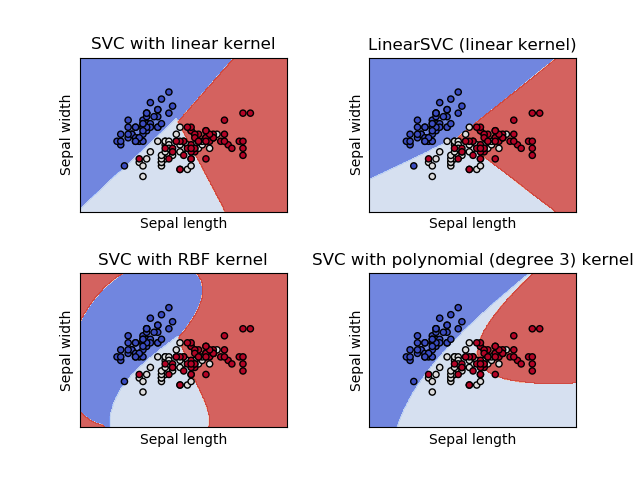
\includegraphics[width=\textwidth]{Figure_1.png}l
\end{figure}
If one were to attempt draw a line that separates the red dots from the blue dots from the white dots, it would be impossible to do so perfectly with a strait line, no matter how it is rotated (figure 1). Luckily, SVM allows for planes to have varying degrees of ``curveyness" based on the gamma parameter. Adjusting gamma can allow the model to be more or less stringent, too little and the model will not perform well, too much and the model will be overfit. Tuning the parameter to the perfect amount is difficult, but can be approximated via bootstrapping/sampling techniques. Another parameter to consider is the `cost'. When drawing the planes that separate the data, SVM first finds the space between different regions where each response category is centered. The space can cary in its `emptyness' depending on the value of the cost. When no points are allowed in between each region, the model is called `hard' and the cost parameter is 0. As the cost parameter is increased, more and more points are allowed to reside in the space between regions. Strict models rarely perform optimally, with many packages defaulting the cost value to 1. After tuning our model with the linear.svc function from the sklearn package, we used a cost parameter of .01. For a more in-depth look at SVM and the underlying math check out (INSERT HERE).(CITE)
To further improve the accuracy of our SVM model within the BBD, we created 100 SVM models from different randomly subsetted training sets, then decided the category of new data via a vote from our 100 different models. This is done in the hopes that diversifying our selection process will aid in classifying borderline data points, and help us identify the structure of difficult to classify numbers.
\subsection{KNN}
The intuition behind K-nearest neighbors (KNN) is quite simple. Consider the following diagram (figure 2). In this case the training data are all the points seen on the plot classified as either red, blue, or green. If one wants to predict what color a new data point will be, an intuitive approach is to look at the data points surrounding the point in question. That is, look at it's nearest neighbors. Determining which neighbors are the nearest involves calculating the distance from the point in question to the other points in the training data set. This creates the colored prediction zones that are shown on the plot. For example, any prediction point that falls in the blue zone will be classified as blue because out of it's 15 nearest neighbors, a majority of them are blue. 

\begin{figure}
\caption{Example of KNN on the python `iris' dataset}
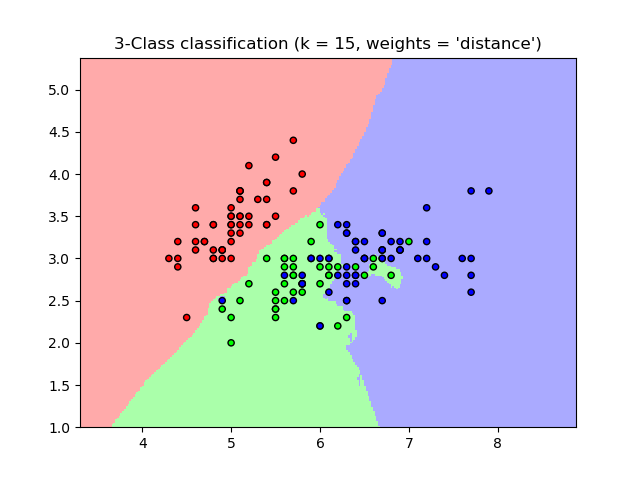
\includegraphics[width=\textwidth]{Figure_2.png}l
\end{figure}
 
That is the essence of KNN, training data is fit to a model, and the response of a new data point is determined by the responses of the k nearest points to the new point. In our case, nearest means smallest Euclidean distance, but other metrics can be used. The points that make up the k-nearest neighbors are called the neighborhood, and can be processed in different ways. The default way is to take the mode category of the neighborhood. Each point inside the neighborhood is asked what its response category is, and the category with the most points determines the prediction of the new point. This way, all points have an equal say in the decision, regardless of how far away they are from C. We decided that the distance between the point in the neighborhood and the new point should have an impact, so our voting scheme is weighted with a gaussian curve. Thus, closer points to the new point have a vote that is worth more than points that are farther away. KNN has some advantages over SVM, one of which is that the only parameter that needs to be tuned is the number of points inside of each neighborhood, k. To find the optimal k, we used the tune function from the FNN package. \cite{FNN} However, since making predicitons often involves looking at many data points and making heavy comptutations (especially for high dimensions), KNN does not effectively make real time predictions. For a more in-depth look into KNN and the underlying math behind it, check out Elements of Statistical Learning, section 13.1. \cite{KNNBook}

\subsection{Random Forest Algorithm}
The Random Forest Algorithm is the only one of the three utilized machine learning techniques that does not take into account all of the predictors all of the time. The principle behind the Random Forest Algorithm is to create N decision trees, and make a decision based on the winner of a vote where every tree gets an equal say. For more information on decision trees, check out Elements of Statistical Learning. \cite{DecisionTree} The number of trees used in each forest is determined based on computing power and possible subsets of the predictors. Decision trees can be overfit if too many predictors are fed through them, but ignoring large swathes of predictors underutilizes the information. The random forest algorithm solves this trade off by randomly subsetting M of the predictors and creating a decision tree based on those predictors, then repeating this process N times. This way, no individual tree is over fit, and all of the predictors are utilized. The number of trees that can be created in our model is bounded by 784 choose M.  It is important to note that many of the predictors in our data set were completely empty, and where thus removed prior to utilizing the model. The parameters to tune in a random forest model are the number of trees (N) and the number of predictors inside each tree (M). Using the estimators function inside the skleanr.RandomForestClassifier package, we decided on a M = 10 and an N = 100. For a more in-depth look into the Random Forest Algorithm and the underlying math behind it, check out Elements of Statistical Learning, chapter 15. \cite{RandomForestBook}
\subsection{Becker-Barton Device}
The thought behind the Becker-Barton Device (BBD) is that the aggregate decisions of many algorithms each playing to their strengths should be more accurate than the algorithms on their own. The structure works by evaluating the certainty of each prediction. Within each algorithm, there are means of evaluating how certain it is about any given prediction. In Random Forest and KNN, this is The thought behind the Becker-Barton Device (BBD) is that the aggregate decisions of many algorithms each playing to their strengths should be more accurate than the algorithms on their own. The structure works by evaluating the certainty of each prediction. Within each algorithm, there are means of evaluating how certain it is about any given prediction. In Random Forest and KNN, this is decided by the ratio of votes, in SVM it is decided by its proximity to the different hyperplanes. The BBD starts with loading in the training data, as well as the 100 SVM models that were pre-trained on subsets of the training data. The other models are then initialized, their predictions are made, and their certainties are calculated. After that, the model looks first to KNN, if it is confident, then it trusts it's prediction. It does the same for the Random Forest algorithm. If neither are confident, it turns to the different SVM models where it will go with the decision with the highest votes. Confidence cutoffs were decided  if there is a tie, it chooses the number with the best track record thus far in our experiments. Below is a visualization of that process. decided by the ratio of votes, in SVM it is decided by its proximity to the different hyperplanes. The BBD starts with loading in the training data, as well as the 100 SVM models that were pre-trained on subsets of the training data. The other models are then initialized, their predictions are made, and their certainties are calculated. After that, the model looks first to KNN, if it is confident, then it trusts its prediction. It does the same for the Random Forest algorithm. If neither are confident, it turns to the different SVM models where it will go with the decision with the highest votes. Confidence cutoffs were decided by finding the minimum percent where the algorithm achieves its maximum accuracy (figure 4, 5). If there is a tie, it chooses the number with the best track record thus far in our experiments. `Track record' was decided by empirical testing on the training data. Below is a visualization of that process. 

% Define block styles
\tikzstyle{decision} = [diamond, draw, fill=blue!20, 
    text width=4.5em, text badly centered, node distance=3cm, inner sep=0pt]
\tikzstyle{block} = [rectangle, draw, fill=blue!20, 
    text width=5em, text centered, rounded corners, minimum height=4em]
\tikzstyle{line} = [draw, -latex']
\tikzstyle{cloud} = [draw, ellipse,fill=red!20, node distance=3cm,
    minimum height=2em]
    \tikzstyle{bblock} = [rectangle, draw, fill=white!20, 
    text width=5em, text centered, rounded corners, minimum height=4em]
\begin{tikzpicture}[node distance = 2cm, auto]
% Nodes
\node at (2.5,5.2) {Becker-Barton Device};
     \node [block] (init) {initialize models};
    \node [cloud, left of=init, node distance=3.5cm] (SVM) {load SVMs};
    \node [cloud, below of = SVM, node distance =1cm] (Train) {load Training};
    \node [block, below of=init] (Fit) {fit predictions, calculate confidence};
    \node [decision, below of = Fit] (KNN) {Is KNN over 65\% conf};
    \node [cloud, left of = KNN, node distance = 3.5cm] (KNNYes) {Use KNN};
    \node[decision, below of = KNN, node distance = 3.5cm] (RF) {Is RF over 60\% conf};
    \node[cloud, left of = RF, node distance = 3.5cm] (RFY) {Use RF};
    \node[decision, right of = Fit, node distance = 4 cm] (SVMMod) {Do SVM models have a winner};
    \node[cloud, right of = SVMMod, node distance = 5cm] (SVMY) {Use SVM vote};
    \node[cloud, right of = KNN, node distance = 7.5cm] (SVMTie) {Use SVM with \\ best record};
    %Edges
    \path [line] (SVM) -- (init);
    \path [line] (Train) -- (init);
    \path [line] (init) -- (Fit);
    \path [line] (Fit) -- (KNN);
    \path [line] (KNN) -- node {Yes}(KNNYes);
    \path [line] (KNN) -- node{No}(RF);
    \path [line] (RF) -- node{Yes}(RFY);
    \path [line] (RF) -- node[near end]{No}(SVMMod);
    \path [line] (SVMMod) -- node{Yes}(SVMY);
    \path [line] (SVMMod) -- node{No} (SVMTie);
\end{tikzpicture}


\section{Results}



The performances of the 3 techniques and the BBD varied to some degree, but all preformed above 96\% accuracy. While this may not compare to some neural network or XGboosting techniques, it is still noteworthy that their most baseline performance was so high. The results are chronicled by the table below:

\begin{center}
\begin{tabular}{ |c|c|c|c| } 
\hline
Model & PCA Prior & Accuracy & Run Time\\
 \hline \hline
  KNN & No &  & \\ 
Random Forest & No &  & \\ 
 SVM & No &  & \\ 
 BBD & N0 &  & \\
 \hline
 KNN & Yes &  & \\ 
Random Forest & Yes &  & \\ 
 SVM & Yes &  & \\ 
 BBD & Yes &  & \\
 \hline
\end{tabular}
\end{center}
\section{Future Work}
As previously mentioned, our techniques, although simple to learn and implement, are not as accurate as some neural networks and the extremely popular XGboosting algorithm. Our future work will consider these two algorithms separately and implement them on our dataset. 

\section{Conclusion}
The KNN, SVM, and Random Forest algorithms all perform at similar levels when analyzing hand-drawn digits. Each method has its advantages as well as pitfalls, and when choosing one over another, one must put serious consideration into run-time. Although the SVM algorithm initially takes a long time to run, once the data is fit, predictions can be made instantly. This makes SVM quite desirable for real time predictions. Since the Becker-Barton Device utilizes all three of these methods, it carries with it all the advantages and disadvantages of the latter three methods. Combining strengths and making predictions based on the model's confidence yields results that are better than using the stand-alone algorithms. This comes at the cost of decreased run time and the inability to make real-time predictions. Mention the best accuracy model. 

%\subsection{}

\begin{thebibliography}{9}

\bibitem{kagglechallange} 
https://www.kaggle.com/c/digit-recognizer, \textit{kaggle, 2018} \copyright
 
\bibitem{kaggledata} 
Kaggle. (1998). Digit Recognizer. Retrieved from https://www.kaggle.com/c/digit-recognizer/data 

\bibitem{PCABook}
he Elements of Statistical Learning, Springer, 2017

\bibitem{FNN} 
Alina Beygelzimer, Sham Kakadet, John Langford, Sunil Arya, David Mount and Shengqiao
  Li (2013). FNN: Fast Nearest Neighbor Search Algorithms and Applications. R package
  version 1.1.
\bibitem{KNNBook}
"13.3 Nearest Neighbor Classifiers." The Elements of Statistical Learning, Springer, 2017, pp. 463?485. 

\bibitem{DecisionTree}
"Decision Trees" The Elements of Statistical Learning, Springer, 2017, pp. 305-315.

\bibitem{RandomForestBook}
"13.3 Nearest Neighbor Classifiers." The Elements of Statistical Learning, Springer, 2017, pp. 463?485.
 
\end{thebibliography}

\end{document}  